\subsection{GPU Background}  \label{GPUBackground}

Figure~\ref{Nvidia680Arch} shows the high-level architecture of the Nvidia GTX Titan Black.
We describe this particular chip because it was used in our experimental evaluation, but also
because it is representative of current GPUs.
In particular, the most recent offering by Nvidia, the GTX~Titan~X uses the same basic Kepler
architecture~\cite{nvidia780}, although the number of cores, memory/cache sizes, and some
micro-architectural details will differ.
%\todo{Is this last sentence still accurate? Yes.}

The GTX Titan Black consists of fifteen \emph{streaming multiprocessors} (SMX), 
each of which contains 192 computing cores, 64K 4-byte registers, 16KB-48KB L1 cache and 16KB-48KB
software managed on-chip memory called \emph{shared memory}, accessible to all cores of the
SMX.\footnote{ 
	Each SMX also contains a texture cache and a constant cache, 
	but they are not relevant for our objectives and hence not considered in this paper.}
A 1.5MB L2 cache is shared by all SMXs, and the L2 cache is connected to
6GB DRAM memory called \emph{global memory}.
We refer to this global memory as \emph{GPU memory} in this paper 
to differentiate it from CPU main memory.
Access latency to registers, L1, shared memory, L2 and DRAM is 10, 80, 80, 240, and 350 cycles,
respectively.
The theoretically maximum bandwidth from L1 (per SMX), shared memory (per SMX), L2 and DRAM have been reported as 180.7GB/s, 180.7GB/s,
1003GB/s, and 336GB/s, respectively~\cite{insideKepler}.
%\todo{Add references, and make sure none of these numbers contradict what we actually were able to measure,}


\begin{figure}
\center
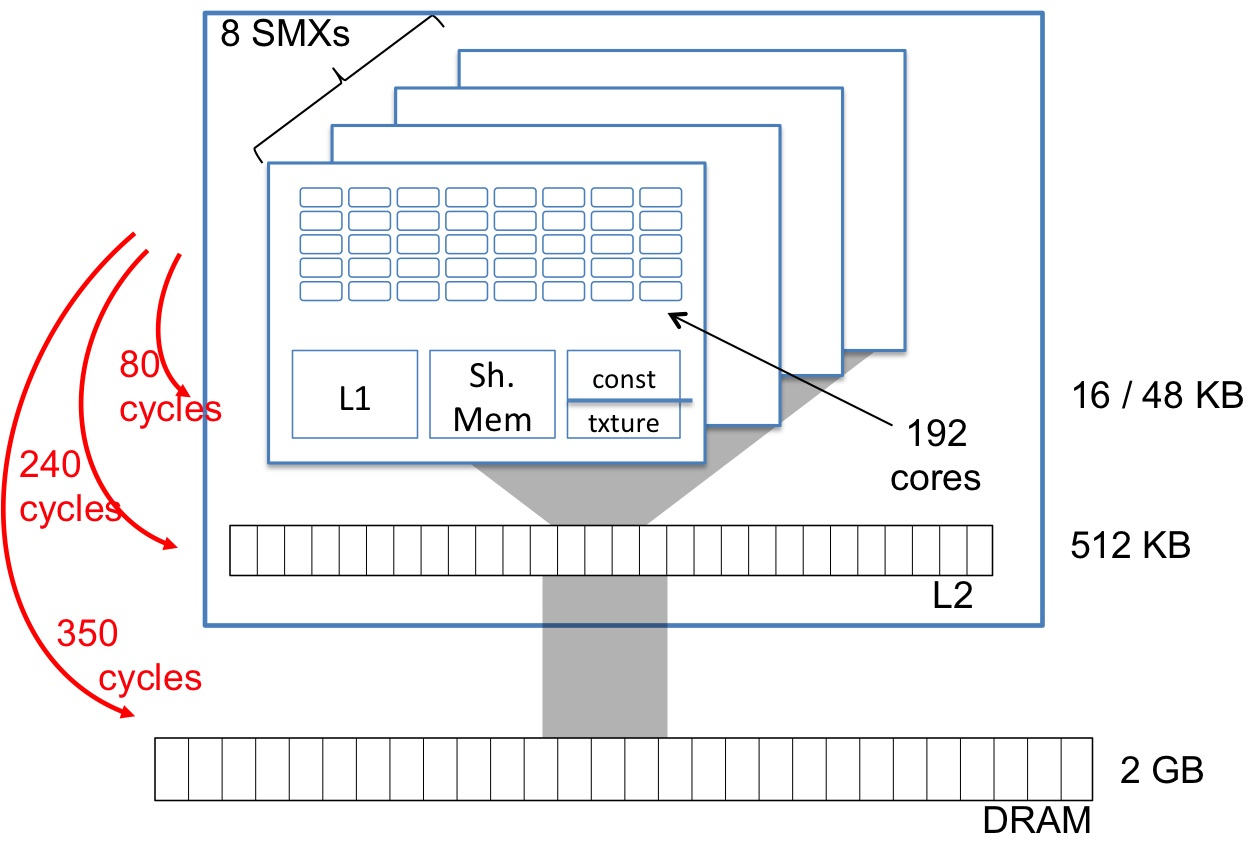
\includegraphics[scale=0.3]{Nvidia680Arch.jpg}
\caption{\footnotesize\textnormal{Architecture of the Nvidia GTX Titan Black.}}
\label{Nvidia680Arch}
\end{figure}

%The GPU is connected to the CPU through a bidirectional PCIe link with 15.75 GB/s maximum throughput in
%each direction.
%The GPU has multiple DMA engines capable of
%transferring data via this link between CPU memory and GPU memory. 
%However, the DMA engine can only access memory CPU-side that has been pinned so that
%it will not be paged out by the operating system.
%The DMA engines also provide GPU cores direct (but slow) access to CPU memory. \todo{We can remove
%this entire paragraph.}

The term \emph{kernel} is used to denote the function that is executed on the 
GPU by a collection of threads in parallel.
The programmer specifies the number of threads to be used,
grouped into {\it thread blocks}, with a maximum
of 1024 threads per thread block.
Each thread block is assigned to a SMX by a hardware scheduler. 
Each SMX can host up to a maximum of 2048 running threads (e.g. two full-sized thread blocks) at a time.

Threads of a thread block are further divided into groups of 32, called \emph{warps}. 
The threads in a warp execute in lock-step 
because groups of 32 cores share the same instruction scheduler.
This lock-step execution will lead to {\it thread divergence} if,
on a conditional branch, threads within the same warp take different paths.
Thread divergence can lead to serious performance degradations. 
%However, inter-warp divergence does not negatively impact performance.

The memory requests issued by threads of a warp that fall within the same aligned 128-byte region are
coalesced into one memory request by a hardware \emph{coalescing unit} before being sent to memory, resulting in only one 128-byte memory transaction. 
Parallel memory accesses from a warp to data are defined as $n$-way coalesced if $n$ of the accesses fall
within the same aligned 128-byte region.




%\todo{Not sure what else would be important here...}
